\documentclass[12pt]{article}
\usepackage{sbc-template}
\usepackage[utf8]{inputenc}
\usepackage[T1]{fontenc}
\usepackage[brazil]{babel}
\usepackage{graphicx,url,booktabs}
\sloppy
\title{Locadora de Veículos: Interface Web Integrada à API do TP1}
\author{Arthur Nunes Henrique dos Santos\inst{1}}
\address{Trabalho Prático 2 -- Sistema de Locadora de Veículos}
\begin{document}
\maketitle
\begin{abstract}
This report presents a web interface integrated into an existing ASP.NET Core vehicle rental API. Five entities support creation, reading, updating and deletion, with server-side filters and relational integrity checks. The implementation preserves the original repository history. Verification results and remaining delivery requirements are explicitly distinguished.
\end{abstract}
\begin{resumo}
Este relatório apresenta uma interface web integrada à API ASP.NET Core da locadora desenvolvida no TP1. As cinco entidades possuem cadastro, consulta, edição e exclusão, com filtros executados no servidor e tratamento das restrições de integridade. O histórico do projeto original foi preservado. São apresentados os resultados verificados e as pendências para a entrega acadêmica.
\end{resumo}
\section{Objetivo e escopo}
O sistema administra clientes, fabricantes, categorias, veículos e aluguéis. O TP2 acrescenta uma interface visual à API do TP1, preservando modelos, migrations, relacionamentos e rotas existentes. A base utilizada foi a revisão \texttt{ea8b138} do repositório original. Antes das mudanças, foi criado um arquivo Git bundle com todo o histórico; o desenvolvimento ocorre na branch \texttt{tp2/interface-validacao}.

Os critérios informados para o trabalho são: CRUD visual das cinco entidades (5 pontos), filtros por pelo menos dois campos por entidade e visualizações (2 pontos), wireframes coerentes (1 ponto) e vídeo entre três e cinco minutos (2 pontos). Há ainda solicitação de relatório em LaTeX no padrão SBC, repositório e ZIP. Os três screenshots do enunciado e da rubrica foram conferidos. A apresentação deve ser um pitch individual de três a cinco minutos, com tela e áudio, sobre o problema, a modelagem e pelo menos duas consultas com seus resultados no front-end.
\section{Arquitetura e integração}
A aplicação utiliza C\#, ASP.NET Core 7, Entity Framework Core 7.0.20 e SQL Server. O front-end foi implementado em HTML, CSS e JavaScript, hospedado na pasta \texttt{wwwroot} do próprio projeto. A ativação de arquivos estáticos em \texttt{Program.cs} permite servir a interface e a API na mesma origem. Não há necessidade de servidor Node.js para executar o produto.

Os formulários enviam JSON por HTTP para os controladores originais. Consultas usam GET, criação usa POST, atualização usa PUT e exclusão usa DELETE. O front-end apresenta mensagens retornadas pela API para erros de validação, conflitos de unicidade, registros inexistentes e relações que impedem exclusão. Conteúdo retornado é inserido como texto, sem interpolação de HTML proveniente do banco.

A navegação organiza as cinco entidades em um menu persistente. As telas contêm título, filtros identificados, contador de resultados e tabela com ações Visualizar, Editar e Excluir. Um diálogo concentra o cadastro e a edição; a visualização desabilita os campos. A exclusão solicita confirmação. Em telas pequenas, o menu e as tabelas permitem rolagem horizontal própria e o formulário passa para uma coluna.
\section{Dados, filtros e relacionamentos}
\begin{table}[ht]
\centering\small
\begin{tabular}{p{2.3cm}p{10.4cm}}
\toprule Entidade & Campos de pesquisa na interface e API\\\midrule
Cliente & Nome, CPF e e-mail\\
Fabricante & Nome e identificador\\
Categoria & Nome e descrição\\
Veículo & Modelo, placa, fabricante e categoria\\
Aluguel & Cliente, veículo, retirada mínima e devolução prevista máxima\\\bottomrule
\end{tabular}
\caption{Filtros independentes, combinados por conjunção quando preenchidos.}
\end{table}
Além dos filtros de cadastro, a tela Consultas do TP1 consome as sete rotas originais: veículos por fabricante, veículos por categoria, aluguéis por cliente, aluguéis por veículo, aluguéis por período, aluguéis por status e fabricantes com veículos. A última utiliza LEFT JOIN e exibe inclusive fabricantes sem veículos. Foram reaproveitados dois fabricantes, uma categoria, um cliente, um veículo e um aluguel fictícios do banco original do TP1, mantendo o original intacto.

Os filtros são parâmetros opcionais nos GETs de listagem. As expressões LINQ são traduzidas pelo EF Core para consultas no SQL Server. O botão Limpar restaura os campos e a listagem. Pesquisas sem correspondência apresentam um estado vazio explícito.

Veículo referencia fabricante e categoria; aluguel referencia cliente e veículo. Os formulários apresentam seletores com nomes e placas, em vez de exigir digitação das chaves estrangeiras. O banco mantém restrições de exclusão e índices únicos para CPF, e-mail e placa. A API valida datas de aluguel, quilometragens, valores, formato dos campos e existência das entidades relacionadas.
\section{Verificação executada}
Em 16 de novembro de 2026, o projeto compilou sem erros com o SDK .NET 9.0.312, mantendo o alvo original .NET 7. O compilador avisou sobre o fim de suporte do alvo; a migração de versão não foi incluída para evitar alterar desnecessariamente a base do TP1.

Foi criado o banco separado \texttt{LocadoraTP2\_Validacao\_20261116}, sem modificar os registros do banco original. As migrations originais criaram as cinco tabelas. A primeira rodada utilizou SQL Server Developer em localhost. Depois da instalação do SQL Server 2022 Express, confirmada por consulta à propriedade Edition do servidor, a mesma bateria ampliada foi repetida no banco separado LocadoraTP2\_Express\_Validacao\_20261116, na instância SQLEXPRESS. As 81 verificações também foram aprovadas nessa edição. Os registros originais do TP1 permaneceram preservados.

O script \texttt{tests/api-integration.mjs} executou 81 verificações HTTP aprovadas: criação, leitura por ID, atualização com nova leitura, filtros positivos e negativos, rejeição de CPF duplicado, dados inválidos, chaves estrangeiras inexistentes, divergência entre IDs da URL e do corpo, resposta 404 e exclusões. A proteção contra exclusão de cliente, veículo, categoria e fabricante vinculados retornou 409. Os registros produzidos pelo script foram removidos em ordem inversa de dependência. O registro completo encontra-se em \texttt{docs/evidencias/api-testes.json}. Mais 16 verificações foram aprovadas para as sete consultas originais, incluindo seus dados fictícios, os resultados de INNER JOIN e LEFT JOIN, parâmetros inválidos e consulta vazia. As sete consultas também foram executadas visualmente no navegador.

Na interface, foram confirmados cadastro e edição das cinco entidades com dados fictícios, incluindo seleção dos relacionamentos em veículos e aluguéis. Também foram observados pesquisa sem correspondências, restauração da listagem e visualização de aluguel com campos bloqueados. Complementarmente, um cliente foi cadastrado pela interface conectada ao Express e sua persistência foi confirmada por consulta SQL direta, registrada em docs/evidencias/sql-express-persistencia.txt. A página foi inspecionada em viewport móvel de 390 por 844 pixels. A confirmação explícita de exclusão foi aberta e cancelada, mantendo o registro. O iniciador de dois cliques foi testado com o servidor desligado: compilou, iniciou a aplicação, preparou os exemplos sem duplicá-los e abriu o navegador. As imagens desta seção são capturas reais da aplicação, e não wireframes.
\begin{figure}[ht]\centering
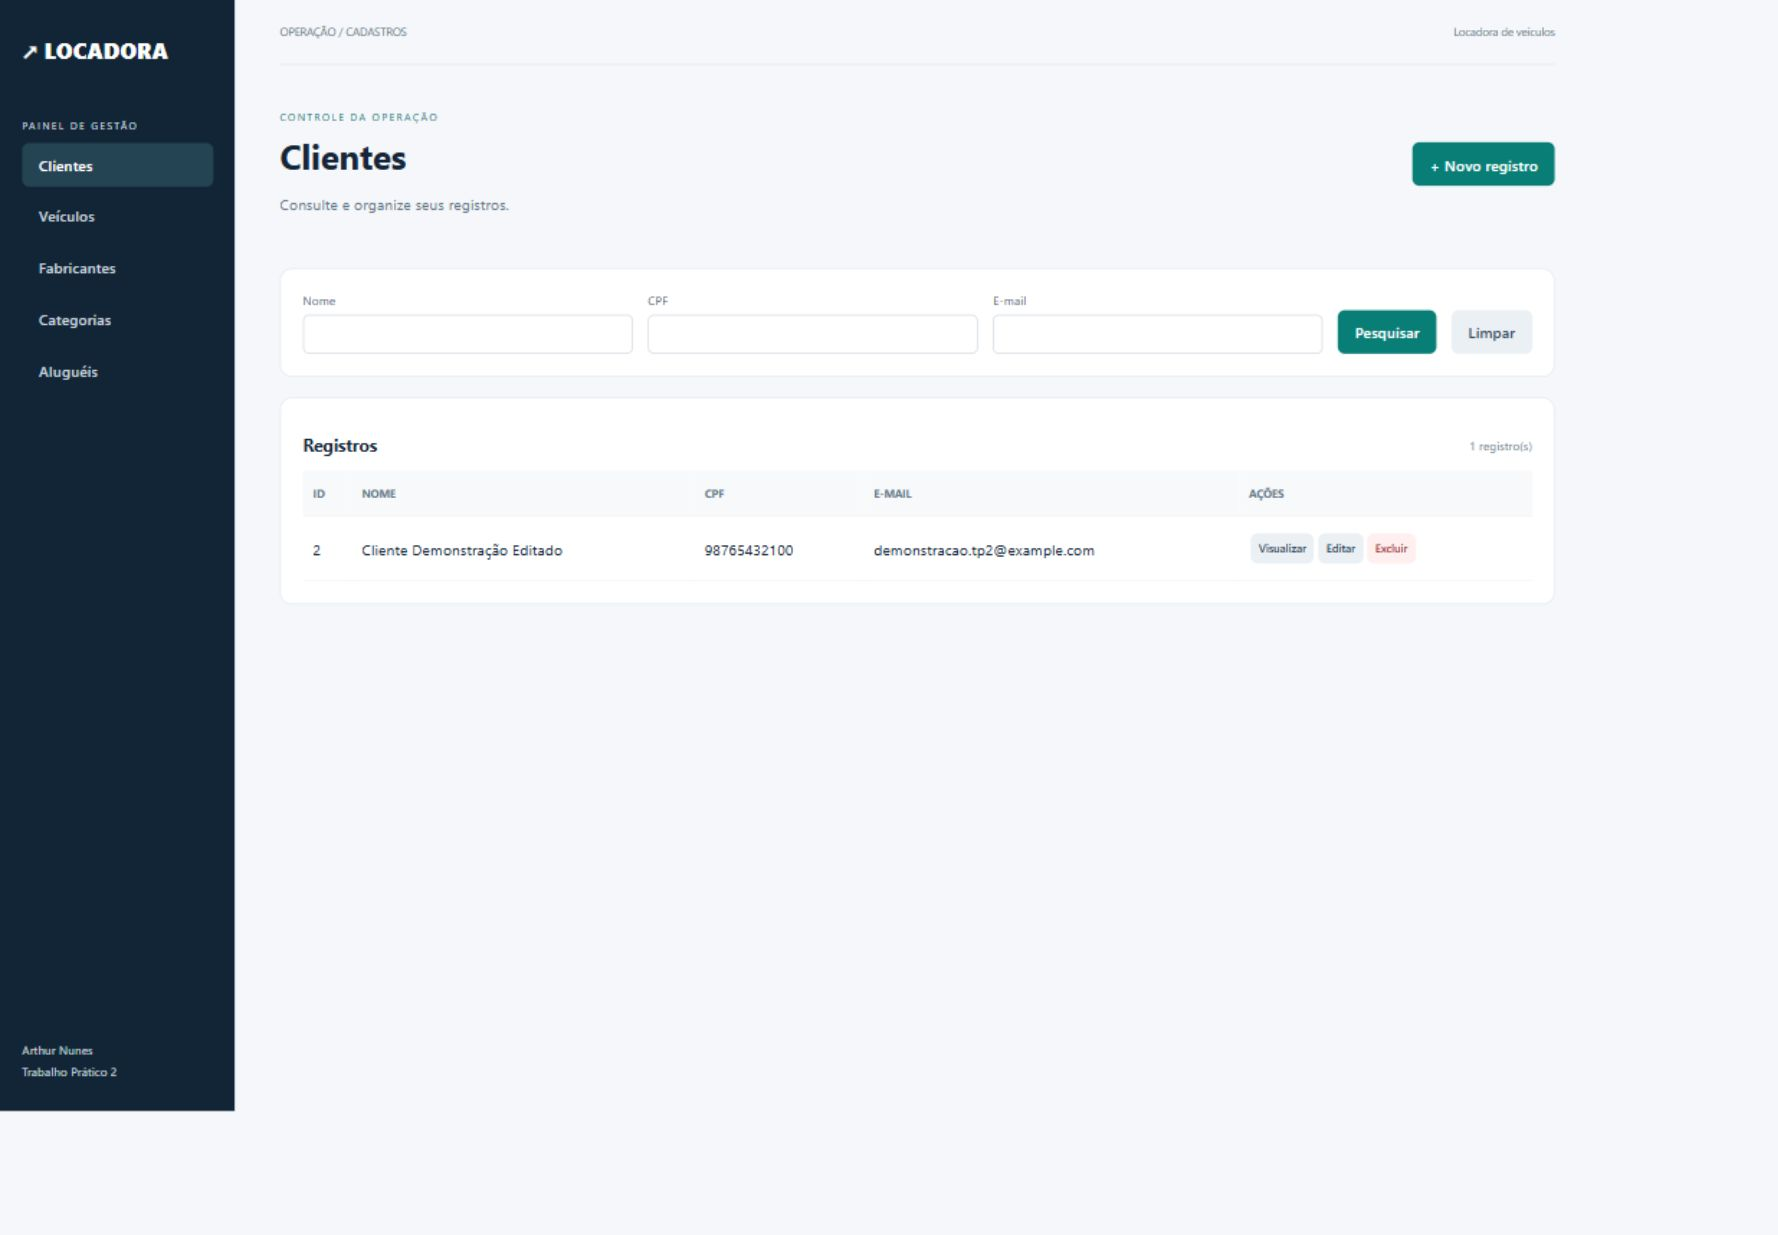
\includegraphics[width=\linewidth]{evidencias/interface-clientes-desktop.jpg}
\caption{Interface real com registro fictício persistido após edição.}
\end{figure}
\begin{figure}[p]\centering
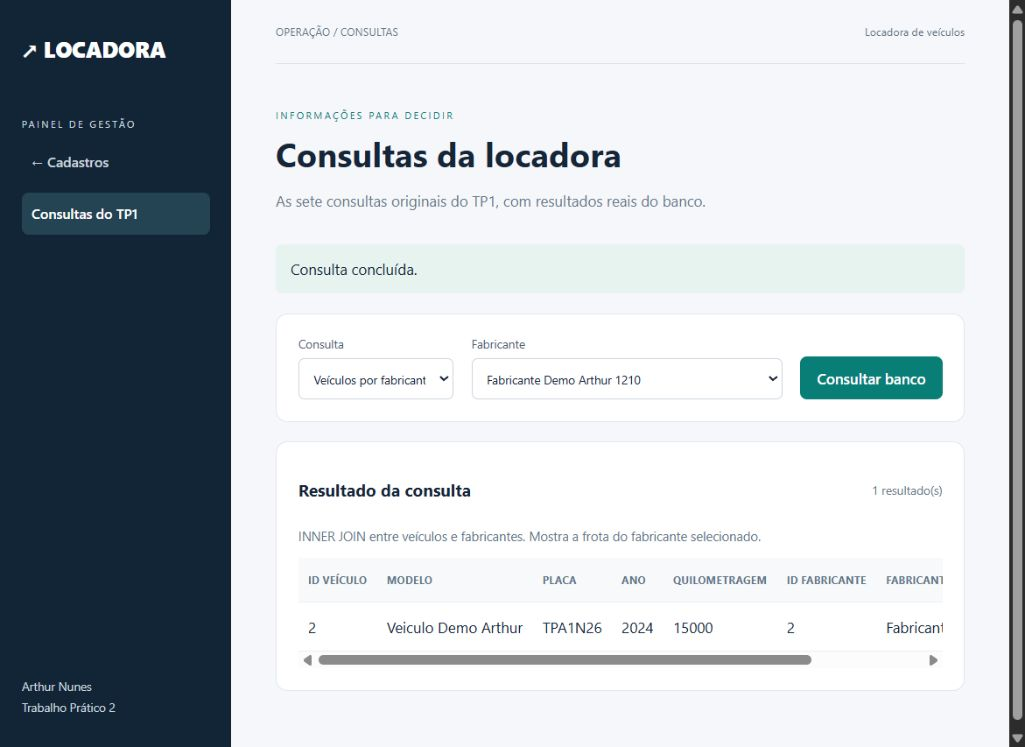
\includegraphics[width=.95\linewidth]{evidencias/consulta-fabricante.jpg}
\par\medskip
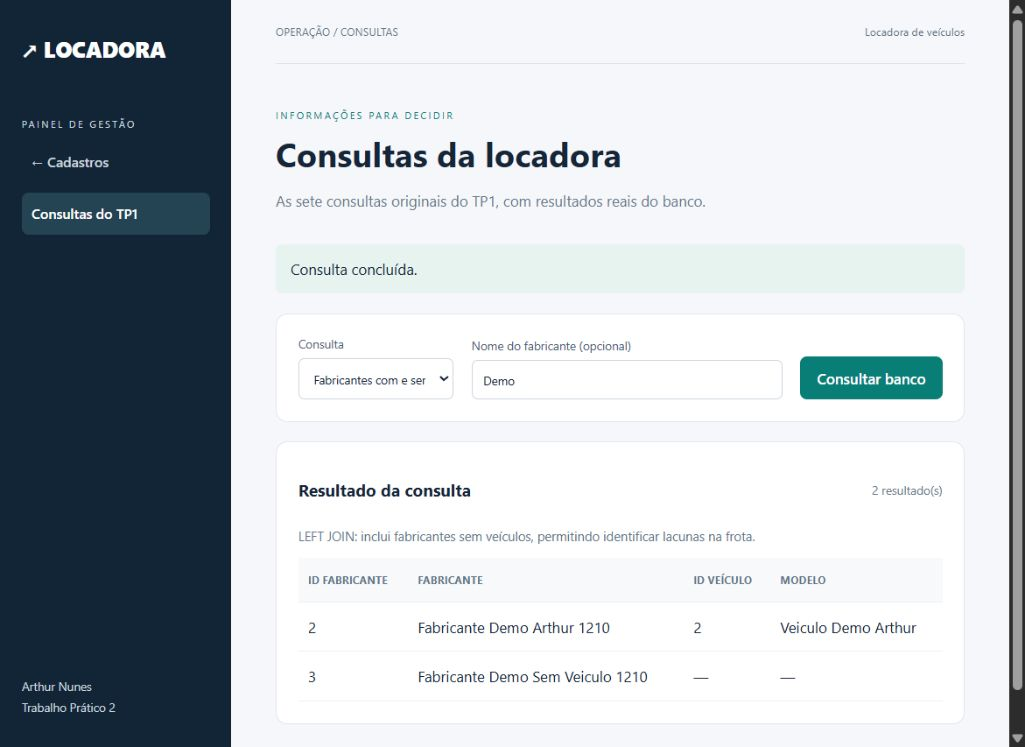
\includegraphics[width=.95\linewidth]{evidencias/consulta-left-join.jpg}
\caption{Duas consultas originais executadas no front-end: veículos por fabricante (INNER JOIN) e fabricantes com ou sem veículos (LEFT JOIN), com exemplos fictícios do TP1.}
\end{figure}
\section{Wireframes e correspondência}
Os seis wireframes SVG na pasta \texttt{docs/wireframes} representam as cinco entidades e a tela de consultas do TP1. O link compartilhável é \url{https://github.com/ArthurBD07/locadora-veiculos-arthur-nunes/tree/tp2/interface-validacao/docs/wireframes}. As visualizações PNG e os SVGs editáveis acompanham o ZIP. Mantêm a organização implementada: navegação à esquerda, título e inclusão no topo, filtros acima da tabela e diálogo de formulário. A versão móvel preserva as mesmas ações, com organização vertical dos campos.

Cliente utiliza nome, CPF e e-mail. Fabricante utiliza nome, com ID disponível na pesquisa. Categoria utiliza nome e descrição. Veículo utiliza modelo, ano, quilometragem, placa, fabricante e categoria. Aluguel utiliza cliente, veículo, datas, quilometragens e valores. As telas de consulta e edição reutilizam a mesma estrutura visual, variando a disponibilidade dos campos e do botão Salvar.
\section{Reprodução e materiais de entrega}
No notebook preparado, dê dois cliques em \texttt{Abrir-Locadora.cmd}. Esse arquivo compila o projeto, inicia o servidor quando necessário e abre \url{http://localhost:5081}. A preparação usa o banco separado do Express e não duplica os exemplos. Para desenvolvimento, abra \texttt{LocadoraVeiculos.sln} no Visual Studio ou execute \texttt{dotnet run --project LocadoraVeiculos} após selecionar o perfil adequado. O perfil SQL Express aponta para a instância nomeada SQLEXPRESS; o perfil SQL Server local aponta para localhost. Em desenvolvimento, o projeto aplica migrations ao banco configurado na inicialização. Para repetir a validação, deve-se selecionar um banco exclusivo de testes e executar o script Node.js indicado.

O roteiro do vídeo está em \texttt{docs/roteiro-video.md}. A gravação \texttt{LocadoraDeVeiculos.mp4} foi recebida em 17 de novembro de 2026 e acompanha o ZIP na pasta \texttt{video}. A imagem mostra a navegação pelos cinco cadastros e duas consultas com resultados: veículos por fabricante e fabricantes com e sem veículos. O arquivo possui resolução de 1920 por 1080 pixels, 30 quadros por segundo e uma faixa de áudio AAC estéreo.

A duração medida é de 5 minutos e 56,36 segundos, superior ao limite de cinco minutos indicado no enunciado. Por solicitação expressa do autor, a gravação foi mantida integralmente, sem cortes, aceleração ou alterações. Sua cópia na entrega foi conferida por SHA-256 e é idêntica ao original. Essa divergência de duração não é apresentada como requisito aprovado. O envio do vídeo e do ZIP ao Canvas, assim como a conferência do vínculo do GitHub com a turma, cabe ao aluno.
\section{Conclusão}
A integração acrescenta acesso visual aos cinco cadastros sem substituir a API original. Os testes automatizados demonstram persistência, filtros e integridade na instância utilizada. O código, os wireframes, a documentação e a gravação foram reunidos para entrega. Permanece registrada a divergência de duração do vídeo, mantido no formato original por decisão do autor, e faltam os envios no Canvas.
\begin{thebibliography}{9}
\bibitem{repo} Santos, A. N. H. Locadora de Veículos. Repositório original. \url{https://github.com/ArthurBD07/locadora-veiculos-arthur-nunes}.
\bibitem{sbc} Sociedade Brasileira de Computação. Template para artigos, disponibilizado pelo SBGames. \url{https://www.sbgames.org/arquivos/Template_SBC/template-latex/}.
\end{thebibliography}
\end{document}
